\documentclass{IEEEtran}
\usepackage[utf8]{inputenc}
\usepackage{graphicx}
\usepackage{subcaption}
\usepackage{url}
\usepackage{amsmath}
\usepackage{wrapfig, framed, caption}

\usepackage{tabularx}
\usepackage{tabularray}
\usepackage[hmargin=1cm]{geometry}

%Dissertation Checklist

%Finish Research Proposal (Few sections missing, sort out citations)
%Ethics Proposal (Done, need to sort out handbook citation)

%Questionnaire (Done)
%Data Analysis Method (Started)
%R-Code (Started)

%Quality Assurance Test Plan (Not Started)

%Presentation (Put hypothesis and more info on how the player model is created)

%Prototype (on defensive actions, check if nearby characters are attacking)

%Useful links
%G-Power downloads
    %https://www.psychologie.hhu.de/arbeitsgruppen/allgemeine-psychologie-und-arbeitspsychologie/gpower
    %https://learningspace.falmouth.ac.uk/mod/resource/view.php?id=245797

\title{Evaluating the use of Adaptive AI to Build Player-Companion Collaboration} 
%Evaluating Collaboration With AI NPCs to Build Player-Companion Relationships
%\title{Does the use of adaptive AI help to build player-companion collaboration?}
\author{Andrew J. Scott}  
\date{September 2022}

\begin{document}
	\maketitle
	\pagenumbering{arabic}

%Careful with the use of I in text, even in abstract. Sometimes we is used, but try to avoid it if possible
%This proposal demonstrates...

\begin{abstract}
This proposal demonstrates the use of adaptive AI for companion characters. The adaptive AI will respond to player actions so it can collaborate with them better. This adaption will be tested to determine if it makes the companion character perceived as more collaborative by the player.
\end{abstract}

 \begin{IEEEkeywords}
Artificial Intelligence, AI, Synergy, Collaboration, Cooperation, Companion, NPC, Adaptive, Game.
\end{IEEEkeywords}

\section{Introduction}
\label{Intro}

This proposal presents an AI companion that will aid the player in combat, similar to \textit{Atreus} in \textit{God of War} or \textit{Ellie} from \textit{The Last of Us}. The focus of this research would be on using agent modelling, outlined in section \ref{Communication}, to make an adaptive AI that determines how the companion can best assist the player without requiring any explicit commands from them.

In the next section, this proposal summarizes the motivations for the project. In section \ref{RelatedWork} , this proposal analyses common design practices for AI. Sections \ref{Responsive Behaviour} \ref{Movement} \ref{ABC} focus on various methods for AI in industry, while section \ref{Communication} focuses on analysing methods in academic research that are used to create adaptive AI. Section \ref{ProposedResearch} details the design of the experiment used in this research.

\section{Background}
\label{Background}

The intention for this research is to provide a framework for developing companion AI that does not rely on using voice acting, writing and animations to make them seem like a real person. The typical approach to developing AI in industry is to focus on these out of combat actions, while the in combat behaviours are less of a focus. For example, \textit{Elizabeth} in \textit{Bioshock: Infinite} interacts with a smart terrain system outside of combat, detailed in section \ref{ABC}. However, her combat functionality is limited to staying out of harm's way and occasionally throwing useful items to the player \cite{GDCElizabeth}.

When developing the AI for \textit{Atreus} in \textit{God of War}, there was a lot more of a focus on the combat AI, but it can be overshadowed as the player can explicitly command the player, which can ruin the companion's agency \cite{EGXCharacterDeathGuildWars}.

This research will build upon combat AI for companion characters by focusing on the sense of collaboration between them and the player. There are five core design pillars:

%List core design pillars
\label{CoreDesign}
\begin{itemize}
	\item \textbf{Enhances Agency} - The AI will have to balance multiple duties, such as helping the player stay safe, attacking other enemies so they do not get overwhelmed and maintaining their own safety \cite{CoupledEmpowermentMaximisation, tremblay2013adaptive}.
	\item \textbf{Doesn't Overshadow} - This AI should not overshadow the player and will use mostly supportive behaviours to assist them \cite{CoupledEmpowermentMaximisation, DesignDocAIAllies}.
	\item \textbf{No Explicit Commands} - Collaboration without explicit commands maintains the companion's own agency \cite{EGXCharacterDeathGuildWars}.
	\item \textbf{Simple Behaviours} - The combat actions for both the player and companion will be simple. This reduces scope and allows the AI to be incorporated in other action games easier. This is standard AI practice in industry \cite{GMTGoodAI, GDCLessIsMore, GDCSimplestAITrick}.
	\item \textbf{Low Maintenance} - While the player should be able to notice the AI, they should not need to rely on them for specific behaviours or completely change their playstyle to get the AI to be helpful.
\end{itemize}

\section{Related Work}
\label{RelatedWork}

Research in 2010 highlights the lack of AI research in games \cite{RealTimeAICritique2010}. Since then, there has been a lot of improvements in AI research. Specifically looking at companion characters, there is a lot of research on implementing adaptive behaviour. Tremblay and Verbugge demonstrate a companion AI that can analyse the player's experience and change its behaviour as a way to dynamically adjust game difficulty \cite{tremblay2013adaptive}.

Friedman and Schrum analysed 2 companion bots in a first person shooter \cite{CompanionBotsFPS2019}. They found that their adaptive AI was not perceived as helpful as the non-adaptive one as the hard-coded agent stayed close to the player and so was seen more in gameplay. However, when shown stats, players tended to state that the adaptive agent was more helpful.

Geib et al. present a plan recognition approach that allows an agent to analyse the actions of another and use those actions to determine what plan is being attempted \cite{GeneratingCollabBehaviourPlanRecognition2016}. Once a plan has been determined, the agent can work through the already completed steps to determine what still needs to be done and take actions towards these steps.

%TODO - cite more reviews and analyses

In industry, games like \textit{God of War 2018}, \textit{The Last of Us} and \textit{Bioshock Infinite} are renowned for their AI companions \cite{PlayDontShow}. All three of the studios behind these games have developed AI techniques to fine-tune behaviour detailed in the next section.

\subsection{Responsive Behaviour}
\label{Responsive Behaviour}

Atreus in \textit{God of War 2018} is a good example of synergistic AI, as he will help the player land slow attacks and will extend enemy vulnerability by shooting them with arrows \cite{GDCAtreus}. For example, when the player launches an enemy into the air, Atreus will shoot them and keep them there. There is also a lot of emphasis on his character development over the course of the game, which is reflected in his behaviour. At the start of the game, he only takes actions when commanded, and learns to be more automated towards the middle of the game. Later, he becomes brash, so he starts to outright ignore the players’ commands, and performs actions that would otherwise only occur when commanded, like his special runic abilities. These changes in his AI help to tie the narrative into gameplay and make him seem like a real character, which helps to allow the player to bond with Atreus. These changes are also noticeable when the player is separated from Atreus, which helps the players realise how much they rely on him.

%Image of pathfinding with caption
\begin{figure}
  \centering
  \includegraphics[width=\linewidth]{Images/TLOUPathfinding.png}
  
\caption{Pathfinding diagram in \textit{The Last of Us}}
\label{fig:TLOUPathfinding}
\end{figure}

\subsection{AI Movement}
\label{Movement}

%TODO - Consider talking about the theatre techniques used in Bioshock: Infinite

Pathfinding is an important aspect of AI companions. The AI needs to be close to the player so that it is not forgotten \cite{GAIP2EllieAI}, but also not too close that it gets in their way and obstructs them \cite{CoupledEmpowermentMaximisation}. An example of poor AI pathfinding is in \textit{Skyrim} \cite{tremblay2013adaptive}, where the AI will move in front of the player when they are aiming and generally get in their way when moving. Naughty Dog addressed these issues in \textit{The Last of Us} with pathfinding tools, shown in figure \ref{fig:TLOUPathfinding}, that keeps companions close to the player, but not in the way \cite{GAIP2EllieAI}. Ellie will also move out of the way if the player moves into her personal space. Vocal barks are used in such moments to add character, and while it is a good practice to use voice acting to help make the player aware of the agent’s actions, and make them feel more real \cite{GMTGoodAI}, they are not suitable for games with lower budgets.

%Images of fight circles with captions
\begin{figure}
  \centering
  
  \begin{subfigure}[a]{\linewidth}
  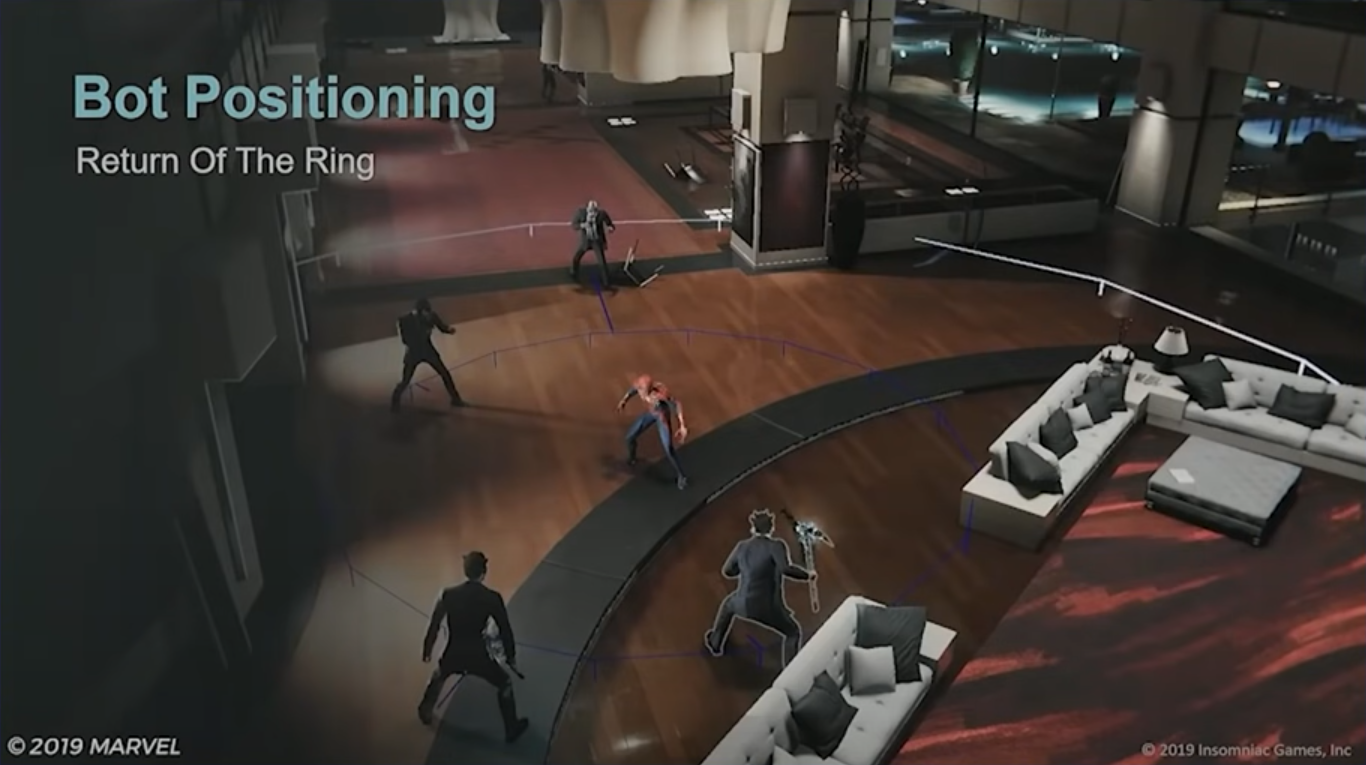
\includegraphics[width=\linewidth]{Images/SpidermanKungFuCircle.png}
  \end{subfigure}
  
  \begin{subfigure}[b]{\linewidth}
  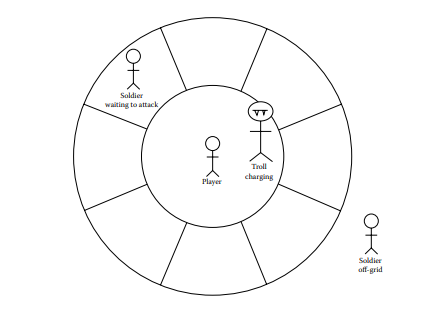
\includegraphics[width=\linewidth]{Images/KOARKungFuCircle.png}
  \end{subfigure}
  
  \caption{Demonstration of Kung-Fu Circles in (a) \textit{Marvel's Spiderman} and (b) \textit{Kingdoms of Amalur: Reckoning}}
  \label{fig:KungFuCircle}
\end{figure}

Many action games, such as \textit{Marvel's Spiderman} and \textit{Kingdoms of Amalur: Reckoning}, use a technique known as the Kung-Fu Circle to manage the positioning of multiple agents \cite{GAIPKungFuCircle, GDCSpiderman}, shown in figure \ref{fig:KungFuCircle}. An AI manager handles the positioning of enemies in this circle and manages when they can attack. While this technique is intended to manage multiple enemies in action games, it can be used to determine where the AI companion could be placed.

\subsection{Animations, Bespoke Behaviours and Call-outs}
\label{ABC}

A lot of industry practice with developing AI for companion characters is to use bespoke behaviour, detailed animations and vocal call-outs to give personality and character \cite{GAIP2EllieAI, GMTGoodAI, GAIPOReactions}. In particular, Irrational Games created a smart terrain system for \textit{Bioshock: Infinite} that allows \textit{Elizabeth} to interact with the environment \cite{GDCElizabeth, AIGamesBioshockAI}, shown in figure \ref{fig:BioshockSmartTerrain}. A lot of these finishing touches are a key part of making the companion feel more believable, allowing the player to empathise and engage with them more. It also helps to communicate NPC actions, so the player understands that they are actually making choices, otherwise they can miss the intelligence of the AI \cite{GMTGoodAI}.

Instead of focusing on animation and voice lines, the agent will use adaptive AI to improve the sense of collaboration between them and the player. The intent of this would be to improve player-companion relationships in games with lower budgets and to maximise them in games that can have animations and voice acting. To do this, it will feature AI techniques that allow a companion NPC to adapt to player actions to collaborate with them better.

\begin{figure}
  \centering
  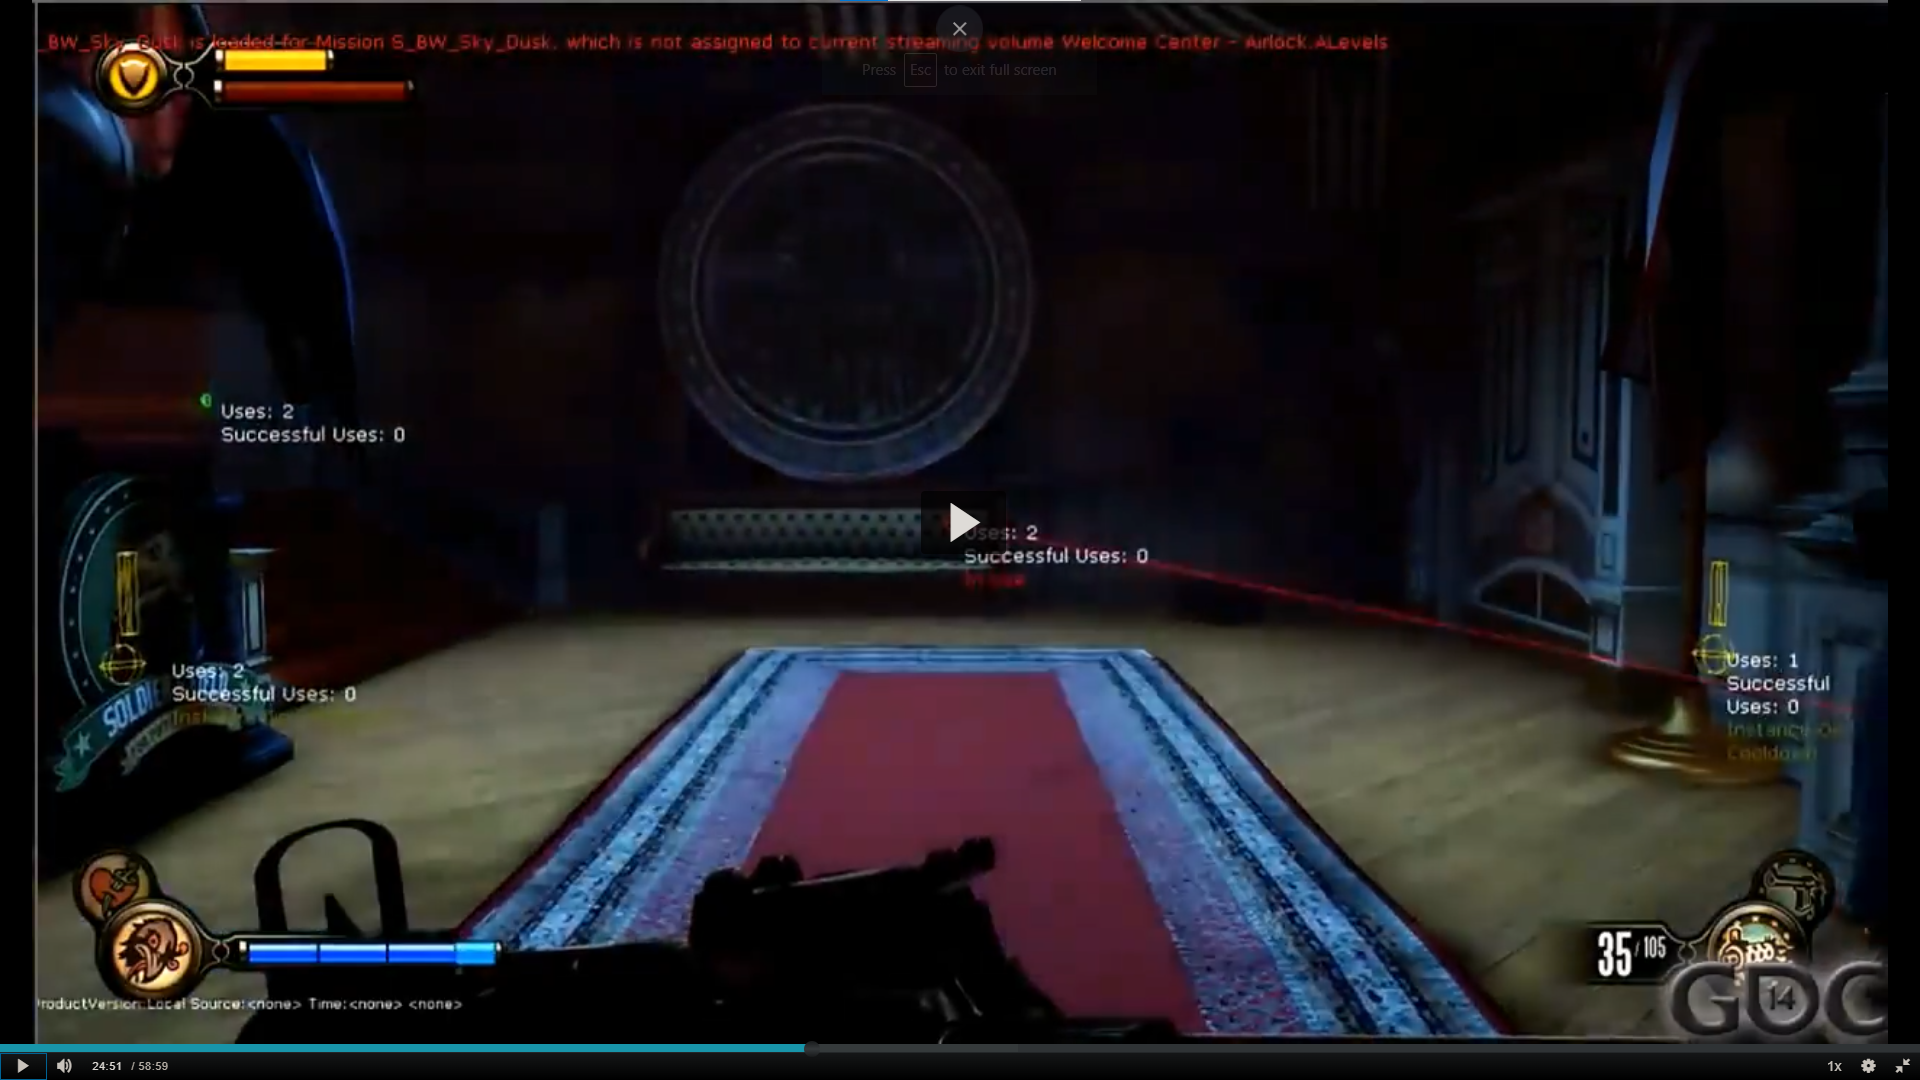
\includegraphics[width=\linewidth]{Images/BioshockSmartTerrain.png}
  
\caption{Smart Terrain showcase in \textit{Bioshock: Infinite}}
\label{fig:BioshockSmartTerrain}
\end{figure}

\subsection{Collaboration Without Communication}
\label{Communication}

The core design, detailed in Section \ref{CoreDesign}, is that the player cannot explicitly command the companion. As a result, the AI needs to determine how to collaborate with the player without communication. The following methods are some ways in which an AI can collaborate with other agents without communication.

Board games like \textit{Hanabi} and \textit{Pandemic} are often used in academic research for collaborative AI as they involve teamwork between multiple players that cannot communicate with each-other. Eger and Grus demonstrate a technique for \textit{Hanabi} that uses timing to communicate between agents \cite{WaitASecond2019}. While this is effective for collaboration between AI agents, this method is not reliable for player-AI collaboration as a human player isn't going to perform actions at specific timings to communicate with an AI agent.

Walton-Rivers et al. present a an AI for \textit{Hanabi} that uses agent modelling to collaborate with other AI players \cite{EvaluatingHanabiAgents}. Agent modelling techniques involve observing actions taken by a player or another agent and using these actions to construct a model of them. This model describes how the observed entity acts and can be used by the AI determine its actions. Yannakakis et al. demonstrate the use of machine learning to determine how an agent can use a player model \cite{yannakakis2013playermodelling}.

Schadd et al. demonstrate the use of agent modelling for \textit{Spring}, a Real-Time Strategy (RTS) game \cite{OpponentModellingRTS2007}. Bakkes et al. then build upon this research to use it in Case-based game AI for \textit{Spring} \cite{bakkes2009opponentmodelling}.

%\cite{van2005opponent} - This tends to not be used for commercial games however (though this source is from 2005 so it may be out of date)

Going back to AI for board games, plan recognition is another common technique that is used in board games. Plan recognition is another useful technique for agents that need to collaborate with other agents, including players, without requiring explicit commands or communication. Agents that use plan recognition observe the actions, similar to agent modelling. However, instead of constructing a model of the player, it uses these actions to their goals by comparing the steps required to achieve that goal to the steps that have been taken \cite{GeneratingCollabBehaviourPlanRecognition2016}. Once an entity’s goal has been identified, the plan recognition agent will devise actions that can aid them in achieving their goals. The unfinished steps in the plan can be used as potential behaviours.

Sauma-Chacón and Eger evaluate the use of plan recognition agents in \textit{Pandemic} that can play with a human player \cite{PandemicPlanRecognition2021}. This AI was able to play at a level similar to that seen in full teams of AI and was perceived as more helpful. In addition, they detected a correlation between perceived helpfulness and skill.

Like agent modelling, this technique can also be used in RTS games as agents use observed behaviour to determine their allies' or opponents' plans. Jansen demonstrates the use of plan recognition as an ally in RTS games, instead of using it as an opponent \cite{PlayerAdaptiveRTSAI2007}. This agent can look at the player's actions and build units to support their plans.

Implementing a plan recognition agent in an action game requires a complex combat system. This type of agent could be useful in an action game with combos, where the AI will be required to determine which attack in the combo the player plans to use, and will plan attacks that collaborate well with them. For example, if the player is building up to a slow attack, they will interrupt enemies from hitting the player and will prevent the target from escaping. If the player is planning a large AOE attack, they will try to stagger enemies into the effect and keep them there. This will ideally make the AI seem intelligent and build collaboration while also appearing to give the AI more agency as it does not respond to player actions directly.

However, these behaviours would be much more reliable with bespoke behaviours, especially since the actions taken by the agent in both examples are quite similar. Using a plan recognition agent in an action game would require the combat system to be complex enough that the agent needs to use unique actions for various plans, which breaks one of the core design pillars outlined in section \ref{CoreDesign}. Looking at Atreus \textit{God of War 2018}, analysed in section \ref{RelatedWork}, all the actions Atreus uses are very similar, but it’s the timing that is important \cite{GDCAtreus}. In addition, these are bespoke behaviours, not a prediction based on what the player is planning.

\section{Proposed Research}
\label{ProposedResearch}

\subsection{Research Question}
\label{ResearchQuestion}

%TODO - Refine research question

The question this research will answer is \textit{Does the use of adaptive AI help to build player-companion collaboration?}

\subsection{Hypothesis}
\label{Hypotheses}

%TODO - Redo this section with new hypotheses and how they will be tested

The hypothesis is that participants that are given the adaptive AI will rate their companion as more collaborative as those without. This means that adaptability has a positive influence on player’s perception of collaboration.

The null hypothesis is that participants that there will be no difference in the ratings for each of the AI companions. This means that adaptability has no discernible effect on player’s perception of collaboration.

%TODO - Fix hypothesis table

\begin{table}[h!]
  \begin{center}
    \caption{\newline{}Hypothesis Table}
    \label{tab:table1}
    \begin{tabular}{|c|c|c|c|}
      \textbf{ } & \textbf{Hypothesis} & \textbf{Null Hypothesis} & \textbf{Data Source}\\
      \hline
      1 & 
      Adaptability makes the companion agent seem more believable & 
      The adaptive agent is not rated as more believable than the non-adaptive agent &
      Questionnaire\\
    \end{tabular}
  \end{center}
\end{table}

\section{Research Method}
\label{ResearchMethod}

\subsection{Philosophical Position}
\label{PhilosophicalPosition}

%What is this thing called Science? https://falmouth.primo.exlibrisgroup.com/discovery/fulldisplay?context=L&vid=44FAL_INST:44FAL_VU1&search_scope=MyInst_and_CI&tab=Everything&docid=alma9911072374905136
%Scientific Method https://plato.stanford.edu/entries/scientific-method/
%Philosophy of Science https://undsci.berkeley.edu/the-philosophy-of-science/
%Philosophy and Paradigm of Scientific Research https://www.intechopen.com/chapters/58890 

The research will be carried out using positivist philosophies \cite{Zukauskas18}. A survey will be used to collect quantitative data that analyses the effect of AI adaptability on the player's collaboration the AI agent, and how that affects their opinions on the AI. There may be some questions with qualitative answers, but these will be used to assure that there are no issues with the study.

\subsection{Experimental Design}
\label{ExperimentalDesign}

%Might be best to have each participant play both as they could be skewed by personal biases so the baseline needs to be established randomise the order

%G-Power video explanation: https://web.microsoftstream.com/video/d1ec1c56-bb97-4592-ae4e-1c973e3fee20?referrer=https:%2F%2Flearningspace.falmouth.ac.uk%2F

Two companion agents will be set up in an action game. The first agent will feature a simple AI which will simply attack the closest target with random attacks and use basic path-finding to keep close to the player when not attacking. The second agent will feature an adaptive AI, which will determine target's based on the player actions and will choose attacks that support the player's intentions better.

Structured observations and questionnaires will be used to collect data on the AI agents. Each participant will fill out an initial survey detailing their experience with games and any general opinions on companions in games.

After completing this survey, they will play through a demo that features two combat encounters. In one encounter, the participant will be assisted by the simple AI agent, while the other encounter will have them assisted by an adaptive AI agent. To avoid priming the participant, the order the agents feature will randomly selected (cite).

%TODO - Citation for priming participants

%https://guilfordjournals.com/doi/abs/10.1521/soco.2014.32.supp.243?casa_token=LllPd7XTs_0AAAAA%3AOjyyDZHutusPSbLINorKbrconK1D2nxtYiADaJjME8mDuTmogdtnsKo-qkZKpETpUsee5w5sDvg)

Once they have played through the demo, the participants will be given a questionnaire form to fill out. Some of the questions would start out establishing the participant's prior experience with games and what kind of games they like, and will then move onto the specifics in the AI.

%TODO - Need more info in this section, talk about required participants, g-power etc.

\subsection{Data Management Plan}
\label{DataManagementPlan}

%TODO - Highlight that I am focusing on perception of AI

Most of the questions will use a Likert scale to distil responses into quantitative data and will include questions on how likeable, intelligent, collaborative, etc. the player thought they were, using a similar approach used by Z. Ashktorab et al. \cite{SocialPerceptions2020}. There will be some qualitative questions that allow participants to put sentence answers so they can give more specific thoughts. This will also help to determine if there are any bugs that caused one AI to not work as intended.

The questions will use a 6-point Likert scale, this means that they will not have a neutral value. This will result in the answer always being useful. Additionally, using a 6-point scale will give more accuracy as it reduces a central tendency bias (cite likert scale). This is caused when participants avoid choosing extreme responses to avoid seeming like they have extremist values. Having a point scale more than 7 may be less manageable for participants

%TODO - More info on the types of questions used, put draft questionnaire in abstract

\subsection{Ethical Considerations}
\label{EthicalConsiderations}

The data collection will involve an experiment that focuses on various AI behaviours, and how different behaviours can build a stronger emotional connection between players and AI companion NPCs. As such, participants will need to be involved. Participants will test the AI and fill out survey forms to give their opinions on the various AI mechanics. Under these criteria, there are no high risk categories, but since participants are involved, it can count as a medium risk experiment.

The participants will be given information forms that detail the experiment and their participation in it. There are no aspects of the experiment that are going to be hidden from the participants, and the form will have clear information on what the experiment will entail. The information form will have the following information as per the Handbook for Research Integrity and Ethics (cite research integrity handbook - 1):

%TODO - citation for the research integrity handbook

\begin{itemize}
	\item The purpose of the research, expected duration, and procedures;
	\item What they are being asked to do;
	\item Their right to decline to participate and to withdraw from the research once participation has begun;
	\item The foreseeable consequences of declining or withdrawing;
	\item Reasonably foreseeable factors that may be expected to influence their willingness to participate such as potential risks, discomfort, or adverse effects;
	\item Any prospective research benefits;
	\item Limits of confidentiality;
	\item Incentives for participation; and,
who to contact for questions about the research. 
\end{itemize}

In order to participate within the experiment, the participant will be asked to sign that they understand and agree with the form, no signature will be required. Participants will also be required to state that they are at least 18 years of age to participate with the experiment. However they will not need to state their age, only that they are above 18 years old. There will also be no transactions or other coercion to participate with the experiment.

All participants will be given a right to withdraw at any time and this will also be made clear in the information and consent forms. The forms will have contact information for them and a reference number so that their responses can be removed without requiring them to give any personal information. They will also be able to use this number to check their responses, though they will not be able to change their results once submitted to preserve pure data.

The questions on the survey forms will not have any questions that require the user to input personal information. The questions are mostly focused on their opinions of the AI, though they may be asked about their opinions on AI in games and how often they play games.

Most of the questions will be using a Likert scale, and there will be few qualitative questions that allow them to express more opinions. None of the questions will require the participants to divulge any personal information. Once the data has been analysed, it will be archived until the study is complete, after which all responses will be deleted.

The experiment will take place on campus, either at the Games Academy Warehouse or the Design Labs and members of staff will be contacted to get permission to use these spaces for the experiment. If there are not enough responses, the project and forms will be sent online to get more responses.

\section{Expected Outcomes}
\label{ExpectedOutcomes}

%TODO - Expected outcomes here

Expected outcomes here
 
\section*{Acknowledgments}

%TODO - Acknowledgements
%Joe, Michael and Liz
%Falmouth Uni
Acknowledgements here

%TODO - Careful with some sources, make sure they are all correct and careful with videos
%TODO - Specify that some are conferences
\bibliographystyle{IEEEtran}
\bibliography{bibliography} 

\section*{Appendix}
\label{Appendix}

%TODO - Appendix

R-code

QA plan

Repo Link

Ethics Proposal

Questionnaire draft

\end{document}